% ********* 中文 ********%%%
% 第4章 设计
\section{Design}

% URN的设计目标是为提供一个统一的RDMA虚拟化框架,以适应混合虚拟化环境,同时实现统一的灵活的RDMA资源管理,并具备与原生RDMA解决的性能。此外,URN应尽可能确保最大的兼容性,对已有RDMA应用透明。
The goals of URN are to provide a unified RDMA virtualization framework for the hybrid virtual environment, meet the unified flexible RDMA resource management and make the performance of virtual RDMA close to the native RDMA meanwhile. Besides, URN should ensure maximum compatibility and be completely transparent to the application. 

%为了实现上述目标,URN主要包含了vRNIC,URN core和mgmt center。vRNIC是对虚拟机和容器通用的虚拟RDMA网卡设备,URN core则是各主机服务器上的用于集中管理RDMA资源的虚拟化层, mgmt center配置各项控制策略。在本章,我们介绍了URN中的一些关键性设计工作。
To achieve the above goals, URN mainly consists of the vRNICs, the URN core and the management center. vRNIC is a virtual RDMA network device that is common to virtual machines and containers, URN Core is a virtualization layer for centralized RDMA resource management on each server, and the management center is configured with multiple control policies. In this section, we introduce some key designs in URN.

% 4.1  vRNIC设计
\subsection{vRNIC}

% vRNIC是一个虚拟RDMA设备,由前后端驱动组成。后端在主机端,模拟RDMA设备;前端在guest端, 作为vRNIC的接口,转发guest应用的RDMA 命令到vRNIC后端。
The vRNIC is a virtual RDMA device that consists of a frontend and backend driver. The vRNIC backend is in the host and emulates the RDMA device in the host. As the interface of vRNIC, the vRNIC frontend is in the guest and forwards the RDMA commands from the upper-level RDMA software to the vRNIC backend. 

% 4.1.1 vRNIC后端
\subsubsection{vRNIC Backend}

% vRNIC后端被放在主机用户空间,因为vRNIC后端在用户空间有诸多好处,具体细节可以见2.1节。
The vRNIC backend is placed in the host user-space, because there are many benefits in user-space, which is discussed in detail at section 2.1.

% vRNIC作为一个虚拟RDMA设备,vRNIC后端需要维护关于RDMA网卡的硬件属性,与物理RDMA网卡对应,例如RDMA地址vGID,RDMA设备类型等。此外,在vRNIC的运行过程中,vRNIC后端中需要维护三方面的上下文:
% 1,来自guest的虚拟RDMA上下文信息,主要记录了虚拟RDMA资源的信息;
% 2,由物理网卡创建的RDMA上下文,包含各RDMA资源,由vRNIC后端利用verbs库创建和维护;
% 3,虚拟RDMA上下文到物理RDMA上下文之间的对应关系。对应关系是一对一的,因为多对一无法实现性能隔离。
As a virtual RDMA device, the vRNIC backend needs to maintain the hardware properties that correspond to the physical RNIC, such as the RDMA address GID, the RDMA device vendor, etc. In addition, three aspects of context need to be maintained in the vRNIC backend at the run-time:
(1) Virtual RDMA context information from the guest, mainly including the information about RDMA resources in the guest;
(2) The RDMA context created on the physical RNIC,  including various RDMA resources, which is maintained in the vRNIC backend with the help of the Verbs libraries;
(3) The mapping between the virtual RDMA context and the physical RDMA context. The mapping of RDMA resources is one-to-one, because shared physical RDMA context cannot achieve the performance isolation.

% 4.1.2 vRNIC前端
\subsubsection{vRNIC Frontend}

% 为了对虚拟机和容器通用,vRNIC前端为不同的虚拟场景提供统一的接口,用于连接guest中的应用和vRNIC后端。虚拟机和容器中有不同的vRNIC前端。 
% 在虚拟机中,vRNIC后端是外部设备,由虚拟机OS中的vRNIC前端驱动。原生RDMA内核驱动包括与设备无关的OFED模块和设备相关的模块,OFED模块接受来自verbs库的命令,提供了内核层级的RDMA API;设备相关模块调用物理网卡设备的硬件接口,执行来自RDMA命令。对应的,在虚拟机中为了使用vRNIC完成RDMA功能,还需要构建一个自定义的设备相关的驱动模块,实现与原生一样的设备相关接口并注册到OFED模块。与原生RDMA不同的是,在这些接口的逻辑中,OFED中的RDMA命令不会在RDMA网卡硬件上执行,而是被转发到vRNIC前端模块,再由vRNIC后端执行。因此,原生的RDMA应用无需修改便可运行在虚拟机中,而且虚拟机内核空间仍然可以使用RDMA。
% 在容器中,vRNIC后端可以和容器应用共享主机操作系统,两者仅位于不同的命名空间。为了在容器的用户空间使用vRNIC,容器的verbs库中与内核RDMA驱动交互的接口,被替换为vRNIC前端接口。Vers库中与内核交互的RDMA命令及参数,被劫持到vRNIC前端。然后通过vRNIC前端转发到vRNIC后端。


% 4.2  URN Core 设计
\subsection{URN Core}

% 为了对vRNIC进行统一管理,高效利用物理RDMA网卡,我们构建了一个统一的虚拟层URN core。URN core部署于集群的每台服务器上,其主要功能包括实例化vRNIC和配置虚拟RDMA网络等。

% 4.2.1 实例化vRNIC 
% URN core在收到虚拟机或容器应用申请vRNIC的请求后,会实例化vRNIC。URN core在实例化vRNIC的主要工作包括: 初始化vRNIC属性、绑定vRNIC到物理网卡、构建vRNIC前后端消息通道以及隔离各vRNIC实例等。

% 初始化vRNIC属性:为了让vRNIC具备与硬件一致的功能接口,URN Core需要对vRNIC的不变属性进行初始化。vRNIC中的不变属性包括RDMA地址vGID,设备号等等。对于RDMA地址vGID,URN core会随机生成IPv6格式的虚拟值,同时通过mgmt center进行协调和登记,以确保各vRNIC的RDMA地址等信息是不冲突的并维护在统一的数据库中。

% 绑定vRNIC到物理网卡:vRNIC实例需要依靠物理网卡实现RDMA功能,因此,实例化vRNIC时需要将vRNIC实例与对应的物理RDMA网卡绑定。如果是多网卡设备或者多个网卡接口(如使用SR-IOV),还需确定从vRNIC到对应物理网卡接口的映射关系。

% 构建vRNIC消息通道:URN Core需要构建vRNIC后端与vRNIC前端(guest)之间的消息通道。对于容器来说,容器与vRNIC后端共享某一IPC命名空间,即可完成vRNIC前端与后端之间的消息交互。对于虚拟机来说,由于vRNIC后端在主机用户空间,而hypervisor位于主机内核空间。为了避免guest的消息先拷贝到hypervisor层再到vRNIC后端,我们在vRNIC后端与guest中的vRNIC前端之间构建一块共享内存,以此作为消息通道。具体来说,虚拟机内存区域对应的物理页面,与vRNIC后端之间是共享的。这样,guest中的任意RDMA消息,均可以直接由vRNIC后端获取,而无需进入到主机内核空间,同时也减少了消息从guest到vRNIC后端的延迟。

% vRNIC实例隔离:URN core需要确保各vRNIC之间的消息通道是隔离的。在云环境中,同一主机上可能部署多个虚拟机或容器,该主机的URN core需要实例化多个vRNIC后端,以满足不同的guest实例。因此,需要确保各vRNIC之间的消息通道是隔离的,尤其是容器,由于其隔离性不如虚拟机彻底。如果多个容器和主机共享同一文件命名空间或IPC空间,那么,很容易通过扫描获取到其他容器或虚拟机vRNIC的消息通道。URN core利用了文件命名空间的机制,文件命名空间中的文件对于其他命名空间是不可见的。URN core在实例化vRNIC时,将各vRNIC消息通道对应的文件位于不同的命名空间,从而实现了各vRNIC实例之间消息通道的隔离。

% 4.2.2 配置虚拟RDMA网络

% URN core在实例化vRNIC后,需要对vRNIC的网络进行配置,包括虚拟RDMA地址配置以及虚拟RDMA路由配置。

% 对于虚拟RDMA地址配置,URN core 在实例化vRNIC时, 给vRNIC配置的vGID是虚拟值,与物理网卡的GID无关。

% 对于虚拟RDMA路由配置,每台主机的URN core中配置了虚拟RDMA网络路由规则。具体来说,URN core在实例化vRNIC时,还给每个vRNIC都配置了组ID,路由规则的定义形式为:{group ID1, group ID2, Policy}。例如,如图4所示,容器1和容器2的vrnic被配置到同一组中,因此允许创建RDMA连接。作为对比,容器1和虚拟机1属于不同的用户组,按路由规则无法建立RDMA连接。各虚拟实例之间建立RDMA连接的具体细节可以参考4.3.1。

% URN core中的虚拟网络配置是动态调整的,因此,容器和虚拟机迁移后无需更改物理网卡及交换机等硬件的网络配置,实现便携的虚拟机或容器迁移。基于URN core中的路由规则,可以支持云环境中的多租户隔离。


\begin{figure}[!ht]
	\centering
	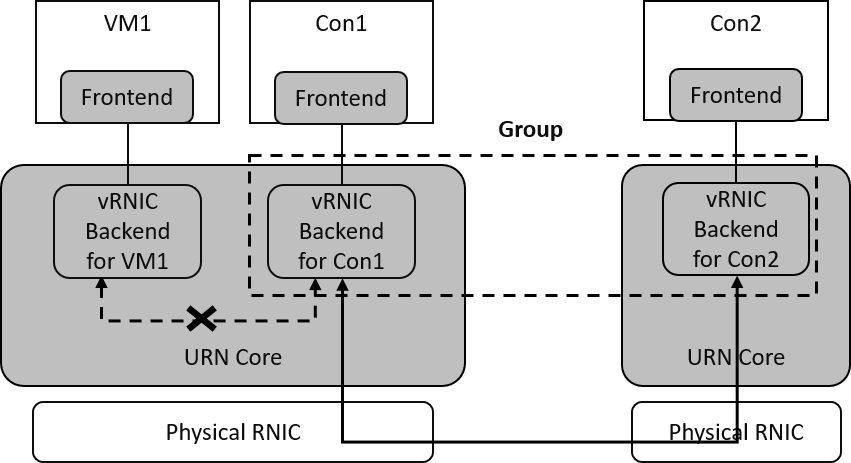
\includegraphics[width=1.0\linewidth]{images/route-config}
	\caption{Group Configuration and Routing: The vRNICs of container 1 and container 2 are configured in one group. Thus, two containers can create RDMA connections. And VM 1 are not allowed to create RDMA connections to containers in this figure because it is not added into the group. }
	\label{fig:route-config}
\end{figure}


% 4.3 虚拟RDMA workflow
\subsection{Virtual RDMA Workflow}

% RDMA的工作流程包括控制路径和数据路径。基于vRNIC和URN core,在虚拟机和容器中可以实现透明的RDMA操作,其中包括控制路径和数据路径。为了实现高性能的RDMA,我们在vRNIC中也采用了控制路径和数据路径分离的设计。其中,控制路径需要经过vRNIC后端,在vRNIC后端中创建RDMA源时会确保资源映射到guest应用。基于映射的RDMA资源,数据路径不需要经过vRNIC后端,直接在guest本地完成,避免了数据路径频繁的拷贝或切换开销。此外,vRNIC在原有的RDMA控制路径中加入了连接管理功能,以适应虚拟机和容器的云环境。

\begin{figure}[!ht]
	\centering
	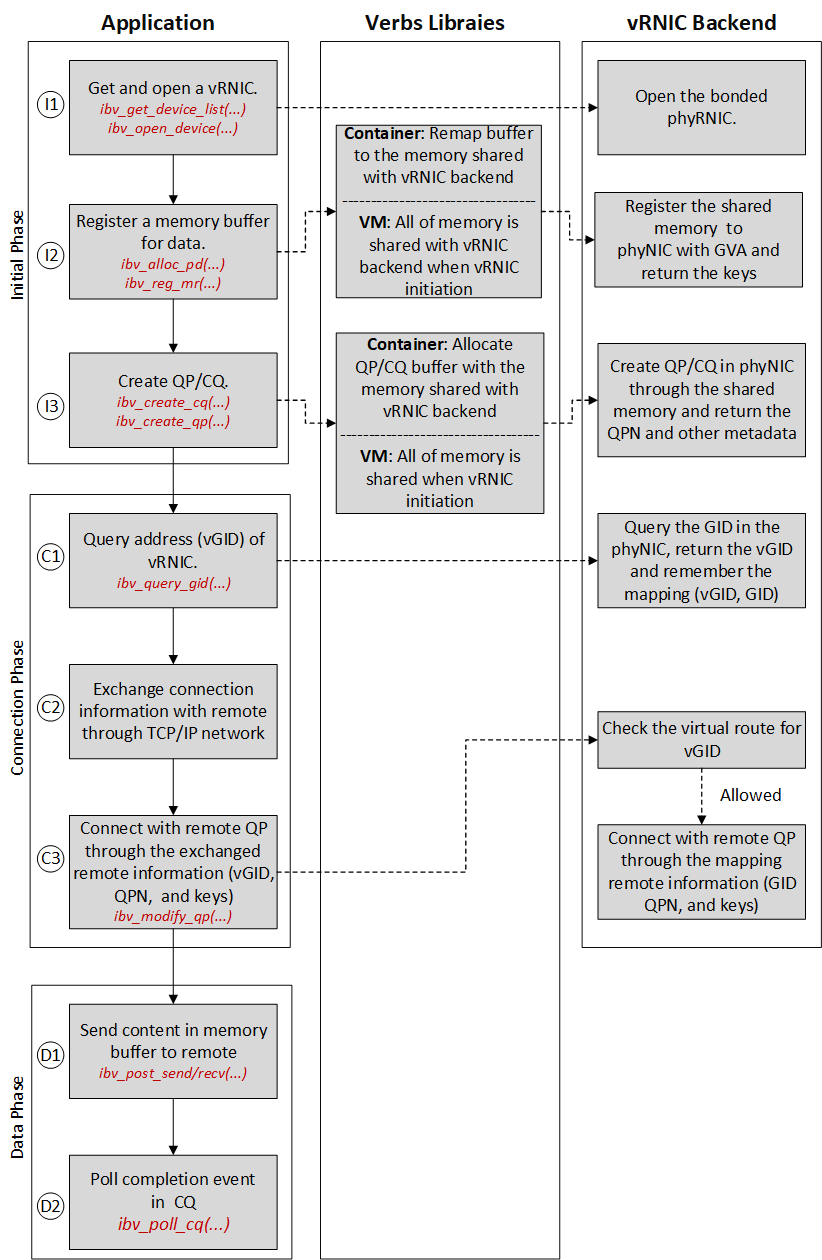
\includegraphics[width=1\linewidth]{images/RDMA-path.png}
	\caption{The Workflow of RDMA SEND operation}
	\label{fig:route-config}
\end{figure}

% 4.3.1 控制路径
%  如图4所示,控制路径依次包括初始化阶段(I1-I3)和连接阶段(C1-C3)。在初始化阶段分别包括设备打开(I1)和RDMA资源创建(I2,I3)。稍后的连接阶段,RDMA应用与远端基于QP与远端建立连接。具体细节如下: 

%(1)初始化阶段
% I1:Guest应用获取并打开vRNIC设备。vRNIC后端会打开在vRNIC实例化时绑定的物理RDMA设备。

%(2)RDMA资源创建和映射
% 按照使用的内存类型,RDMA资源分为主存资源(使用物理内存,如QP)和设备资源(使用设备内存,如门铃)。
% 对于主存资源(如QP,CQ和MR),在创建资源的过程中完成资源映射操作。无论是虚拟机还是容器,这类资源映射都是基于共享内存的方式来完成。具体如图4所示:

% I2:Guest应用注册MR。由于MR的内存区域是由应用指定的,为了让MR的内存和vRNIC后端完成映射,同时维持URN对应用的透明性,我们修改了容器的Verbs库,将应用指定的MR内存重新映射到某一共享内存,然后将该路径随MR命令及参数传递到vRNIC后端。
% 对于虚拟机,由于vRNIC在实例化时,vRNIC后端已经和虚拟机的整块内存完成了共享,虚拟机中的Verbs库此时无需额外映射工作。vRNIC后端在收到该命令及参数后,会使用对应的共享内存注册MR,并返回MR内存地址(s-hvm)和key等信息,在虚拟机和容器的Verbs库中,则会记录guest中MR内存地址(gvm)与s-hvm,以及MR的key,这三者的对应关系,用于后续的数据路径操作。

% I3:Guest应用创建QP/CQ等RDMA资源。原生RDMA中QP/CQ内存的分配是硬件相关的用户库中进行的,该库中对于QP/CQ等RDMA资源内存的分配方式并未包括共享内存。因此,为了让QP和CQ内存和vRNIC后端之间完成映射,同时避免修改Verbs库与应用交互的Verbs API(例如ibv_create_qp, ibv_create_cq),我们在硬件相关的用户库中增加了基于共享内存分配RDMA资源的函数,例如alloc_shm_buf,通过该函数分配好QP/CQ内存后,对应的共享内存路径会随RDMA命令和参数传递到vRNIC后端。
% 对于虚拟机,由于vRNIC实例化是vRNIC后端已经共享了虚拟机的整块内存,无需这一步骤。
% vRNIC后端在收到这些命令和参数后,在创建QP/CQ时,其分配的内存需是与虚拟机或容器共享的内存,此时,仍需修改设备相关的用户库,主要增加了基于指定内存地址分配QP/CQ等RDMA资源内存的函数,例如alloc_assigned_buf。在创建资源后,vRNIC后端会返回QPN等RDMA资源的元数据。 
% 总之,对于QP/CQ等RDMA资源,Verbs库和RDMA设备相关用户库对RDMA虚拟化的支持不够,未考虑到使用共享内存映射RDMA资源的情形。为此,我们建议Verbs库或设备相关库中增加以下API,以加强对各场景下RDMA虚拟化的支持,如下表所示:
% API  所属库  功能 
% alloc_shm_buf()  设备相关库 创建并分组共享内存作为RDMA资源内存
% alloc_assigned_buf(addr, size) 设备相关库 为RDMA资源指定某一内存区域
% ibv_create_qp/cq_shm() 基于共享内存区域创建QP/CQ
% ibv_assigned_qp/cq 使用指定的内存区域创建QP/CQ

% 对于设备资源(如门铃),它位于设备地址空间,由RDMA设备驱动管理。因此,无法在用户空间完成映射。为此,我们设计了一个用于映射RDMA设备资源且与host端RDMA内核驱动解耦的内核模块。vRNIC前端会将设备资源映射的命令和地址参数,转发到一个host内核模块,由该模块完成映射操作。具体细节见实现章节。 

%(3)虚拟RDMA连接建立

% C1:Guest应用查询vRNIC的vGID地址。vRNIC后端会获取绑定的物理RDMA网卡的GID,并记录(vGID,GID)对应关系。不过,vRNIC后端返回给guest的仍然是vGID。

% C2:Guest应用与远端RDMA连接所需的地址信息vGID,QPN和MR key等。 该步骤完全由应用程序完成,无需调用Verbs库。例如,应用中可以使用TCP socket来与远端guest应用完成这一系列信息的交换,
%  C3:Guest应用使用本地QP,基于远端vGID,QPN等信息与远端QP建立连接。该命令需要转发到vRNIC后端执行。vRNIC后端会先根据设置的路由表规则进行判断,如果远端vGID符合路由规则,就会将vGID转换成对应的GID,基于GID,QP ID及Key完成与远端vRNIC后端QP的配对。从vGID到GID的转换,实现了RDMA连接的网络虚拟化。
% 第七步:Guest应用将QP修改为连接状态,两端RDMA连接建立。在完成配对后,该命令会转发到vRNIC后端,由后端基于物理RDMA网卡的QP执行。由于QP在前面的第二步中已完成映射,在vRNIC后端QP处于连接状态后,guest中的QP同样会处于连接状态。

% 4.3.2 数据路径

% 数据路径发生在连接建立后,主要操作注册的MR中的内容。RDMA的数据路径包含双边操作(Send/Recv)和单边操作(Read,Write)等多种数据操作。数据路径主要包括了图中的第8和9步。

% (1) 双边操作
% D1:Guest应用发送MR中的数据。由于MR和QP已经完成了资源映射,此时,数据操作时的数据块(MR中)和工作请求(QPs)可以直接由RDMA物理网卡访问。不过,工作请求中的地址信息仍然是guest中的地址,而第三步中创建MR时,物理网卡记录是vRNIC后端中的页表信息。因此,需要借助前面缓存的三元组信息,将工作请求中的guest地址转换为vRNIC后端地址,再填充到QP中。
% D2:Guest应用轮询CQ获取数据操作的完成事件。由于CQ已经完成了资源映射,此时,物理网卡中工作完成的通知会直接写入到guest的CQ中。

% (2) 单边操作
% 单边操作中,第八步和第九步仅在已建立RDMA连接的一端执行。单边操作的工作请求中包含了远端guest MR的内存地址及key,该信息在第五步已经由两端guest应用完成交换。由于远端应用注册MR时,其RDMA网卡中在缓存的是远端vRNIC后端的页表, 单边操作还需要知晓远端vRNIC后端的MR内存地址。为此,我们建立了一个分布式的KV数据库,存储各节点注册MR的映射关系。在guest执行单边操作时,将向分布式KV数据库查询,以获取远端vRNIC后端的MR内存地址,将其写入单边操作的工作请求中,从而实现单边操作。然而,由于频繁地查询分布式KV数据库会带来较高的延迟,为此,我们利用了RDMA数据收发的局部性,在guest本地建立了一个KV缓存区,以加速单边操作的性能。


% 4.4 mgmt center
\subsection{Management Center}

% 在URN框架里,整个集群配备一个mgmt center,作为配置管理策略,存储各节点RDMA资源信息的中心。

% 通过mgmt center,管理者向不同节点的URN core下发各种策略,包括控制平面和数据平面。管理框架图如图5所示。
%  在控制路径:控制路径可以实现的管理功能包括路由管理、防火墙等。这些策略主要依靠RDMA资源,如QP进行控制。具体地,vRNIC后端按照mgmt下发的策略,可以在创建RDMA资源前执行策略,并在策略执行后将结果或资源信息返回给mgmt中维持各RDMA上下文信息的数据库中。
%  在数据路径:云环境中需要更多的管理功能,例如QoS,流量计费等策略。显然,这些策略依赖RDMA中数据路径的信息,例如消息大小。然而,在URN中,vRNIC前端和后端都在数据路径中被绕过。因此,我们应该将这些管理扩展到guest中的特定硬件库中,因为数据路径是在这个库中实现的。对于策略,可以通过管理中心进行配置和分发。注意,这些扩展需要所有客户机都信任库,并且这些修改应该包含在TCB(可信计算库)中。

% 4.5 discussion
\subsection{Discussion}

%  (1)虚拟机迁移: 容器或虚拟机迁移在云中有很多好处,例如资源利用和故障转移。通过使用虚拟RDMA网络,URN可以支持脱机迁移,而无需为应用程序重新配置物理RDMA网络。具体来说,在重新启动迁移的虚拟实例后,应用程序可以通过相同的网络地址重建RDMA连接。唯一的工作是修改URN core中的地址映射.目前,由于RDMA应用程序中的内存区域在旁路或单侧通信下可能存在不确定性,因此对动态迁移仍然存在困难,URN 并未不会引入更大的困难.
 Virtual Instances Migration: Migration of containers or VMs has many benefits in clouds, e.g. resource utilization and fail-over. With the virtual RDMA network, URN can support offline migration without reconfiguring the physical RDMA network for applications. In specific, after rebooting the migrated virtual instance, the application can rebuild the RDMA connection through the same network address. The only work is modifying the address mapping in URN core. Currently, for live migrations, it is still hard because memory regions in RDMA application may be uncertain under bypassing or one-side communication. And the problem is unrelated to URN.
%%%*********************%%%
